\documentclass[11pt,a4paper]{article}

\usepackage[utf8]{inputenc}
\usepackage[T1]{fontenc}
\usepackage{lmodern}
\usepackage[english]{babel}
\usepackage[a4paper,margin=2.3cm]{geometry}
\usepackage{microtype}
\usepackage{graphicx}
\usepackage{booktabs}
\usepackage{tabularx}
\usepackage{array}
\usepackage{enumitem}
\usepackage{xcolor}
\usepackage[font=small,labelfont=bf]{caption}
\usepackage{float}
\usepackage{amsmath}
\usepackage{xurl}
\usepackage[hidelinks]{hyperref}
\usepackage{fancyhdr}
\usepackage{tikz}
\usetikzlibrary{positioning,arrows.meta,fit,calc}
\tikzset{
  box/.style={rounded corners=2pt,align=center,font=\footnotesize,minimum height=8mm,inner sep=3pt},
  blk/.style={box,draw=accent,fill=accent!8},
  new/.style={box,draw=orange!80!black,fill=orange!12},
  hw/.style={box,draw=black!55,fill=black!7},
  grp/.style={draw=black!40,dashed,rounded corners=4pt,inner sep=6pt},
  grplabel/.style={font=\scriptsize\itshape,text=black!60,anchor=south west,inner sep=1pt},
  lab/.style={font=\scriptsize,text=black!75},
  arr/.style={-{Stealth[length=2mm]},thick,black!70},
  fb/.style={-{Stealth[length=2mm]},thick,dashed,red!70!black},
}

\definecolor{accent}{HTML}{256ABF}
\hypersetup{colorlinks=true,linkcolor=accent,urlcolor=accent,citecolor=accent}

\setlist{itemsep=2pt,topsep=4pt}
\setlength{\parskip}{4pt}
\setlength{\parindent}{0pt}
\renewcommand{\arraystretch}{1.2}
\newcolumntype{L}{>{\raggedright\arraybackslash}X}

\pagestyle{fancy}
\fancyhf{}
\lhead{\small Hash assembly with two xArm6 robots}
\rhead{\small ETH Zurich, am|z -- technical assignment}
\cfoot{\small\thepage}
\renewcommand{\headrulewidth}{0.4pt}

\newcommand{\code}[1]{\texttt{#1}}
\newcommand{\repo}{\url{https://github.com/David543M/eth-hash-assembly}}

\begin{document}

\begin{titlepage}
\vspace*{3cm}
{\Large\textcolor{accent}{Technical assignment}}\\[6pt]
{\LARGE\bfseries Hash Assembly with Two UFACTORY xArm6 Robots}\\[10pt]
{\large Pick-and-place set-up, simulation and a strategy to meet the drawing tolerances}\\[1.5cm]

\begin{tabular}{@{}ll}
Position & Scientific Assistant in Industrial Robotics and Manufacturing\\
Lab & Advanced Manufacturing Lab (am|z), ETH Zurich\\
Drawing & AMZ-SA-26-001 rev.\ A\\
Author & David\\
Date & 8 November 2026\\
Repository & \repo\\
\end{tabular}

\vfill
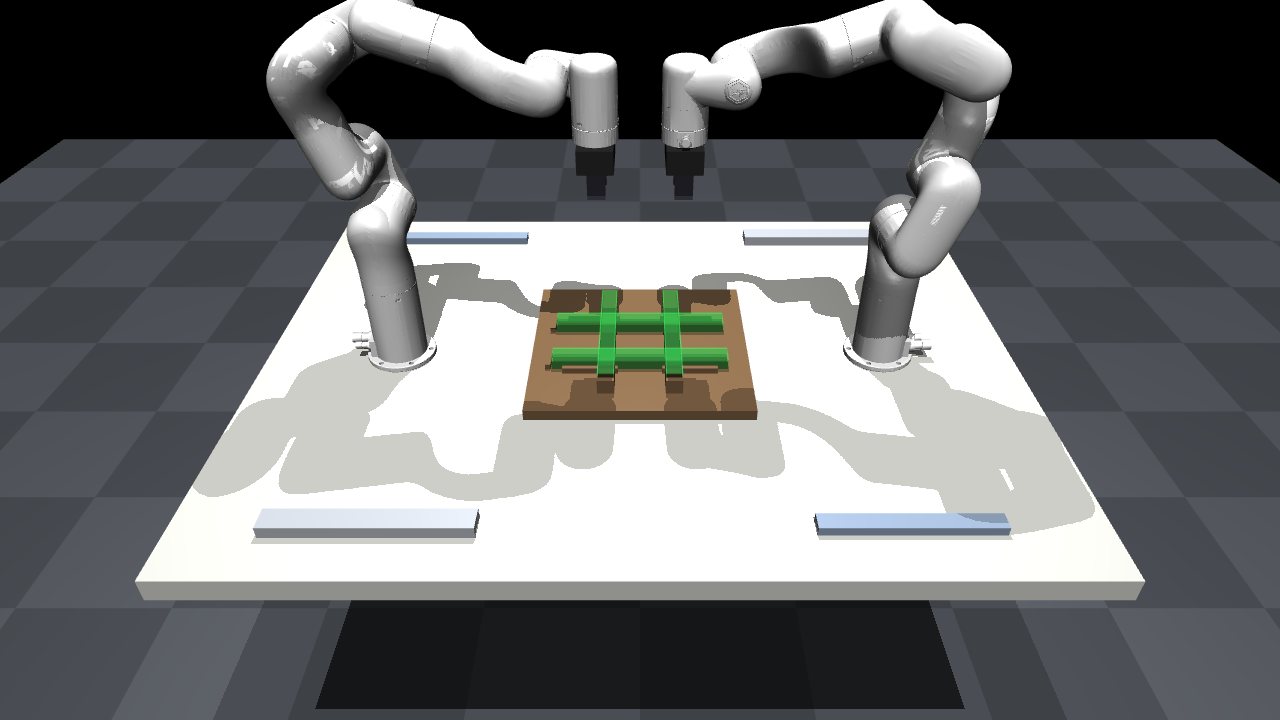
\includegraphics[width=\textwidth]{figures/scene_overview.png}
\end{titlepage}

\tableofcontents
\vspace{1em}

%==============================================================================
\section*{Summary}
\addcontentsline{toc}{section}{Summary}

\textbf{Context and problem:} 

Two UFACTORY xArm6 arms are to pick up four U-profiles into a
hash-shaped part as specified in the technical drawing that asks for $\pm0.05$\,mm positions tolerances and 0.05\,mm geometric tolerances. 
That is half the robot's $\pm0.1$\,mm repeatability and far below its absolute accuracy which is not published. 
That is why the key question is not only how to automate this assembly process, but also how and under what conditions these tolerances can be met if the robots themselves are not capable of doing so.

\textbf{Approach:} 

To tackle this problem, the cell, the two robots and their assembly cycle were simulated using the MuJoCo physics simulation software; the code is written in Python, a hardware abstraction layer is used to facilitate the transition to the physical environment, and 15 tests are automated via continuous integration to verify that the code produces the correct result.

Next, the kinematics and singularities of the xArm6 arms were analysed.

A Monte Carlo simulation analyses the tolerances of 100\,000 assemblies per scenario.

The scenarios range from free placement by the robot to a fully fixtured process.

\textbf{Key results:} 

The results obtained include a cycle time of 32 seconds for both robots.

Dexterity is increased fivefold by moving the magazines 300 to 450 mm away from the base to move them clear of a ring of quasi-singular wrist positions.

The parts released by the robot land, on average, 0.7\,mm from the nominal value,
meaning that the robot alone never produces a compliant assembly, whereas a self-centring fixture ensures compliance with five of the eight characteristics (A1, A2, A5, A6, A8). 

The other three characteristics are determined by the parts themselves: the closed chain $100 + 120 + 100 = 320$ requires part lengths
within a tolerance of approximately $\pm0.1$\,mm, whilst the drawing permits $\pm0.5$\,mm (ISO 2768-m).
A4 specifies a width of $\pm0.3$\,mm from position 1, and the upper parallelism (A7) depends on the difference in height
between the two positions 1.


\textbf{Conclusion and recommendations:} 

Tolerances can only be met if the accuracy stems from the process rather than the robot: a self-centring clamping device, Pos~1, height-matched, assembly under clamping and the machining of the ends referenced on the Pos~2 axes ensure 100\,\% on axes A1 to A6 and A8, whilst axis A7 remains the limiting factor (71\,\%) and requires either a height selection or a review of this tolerance with the designer. These figures are derived from models and must be confirmed on actual parts, in accordance with the commissioning plan in section~\ref{sec:sim2real}.

\textbf{Deliverables:} 

The deliverables include this report, a Git repository (\repo) containing the cell model, the
two-robot cycle, the tolerance model and 15 automated tests run in CI, a video of the cycle
(\code{docs/cycle.mp4}) and the specifications.

%==============================================================================
\section{Drawing analysis}

The assembly consists of a two-level ‘lattice structure’ formed from four cold-formed S235JR (EN 10162) U-sections, all
with the flanges facing downwards: two Pos~1 (U\,40$\times$20$\times$2, L\,320, 0.38\,kg) on the base plate and two
Pos~2 (U\,30$\times$15$\times$2, L\,280, 0.25\,kg) arranged transversely. The tolerances of the parts comply with ISO 2768-m:
$\pm0.5$\,mm on the lengths, $\pm0.3$\,mm on 40, $\pm0.2$\,mm on 15, 20 and 30. No assembly method
is specified. The drawing is reproduced in Figures~\ref{fig:drawing} and~\ref{fig:drawing-parts}.

\begin{figure}[H]
\centering
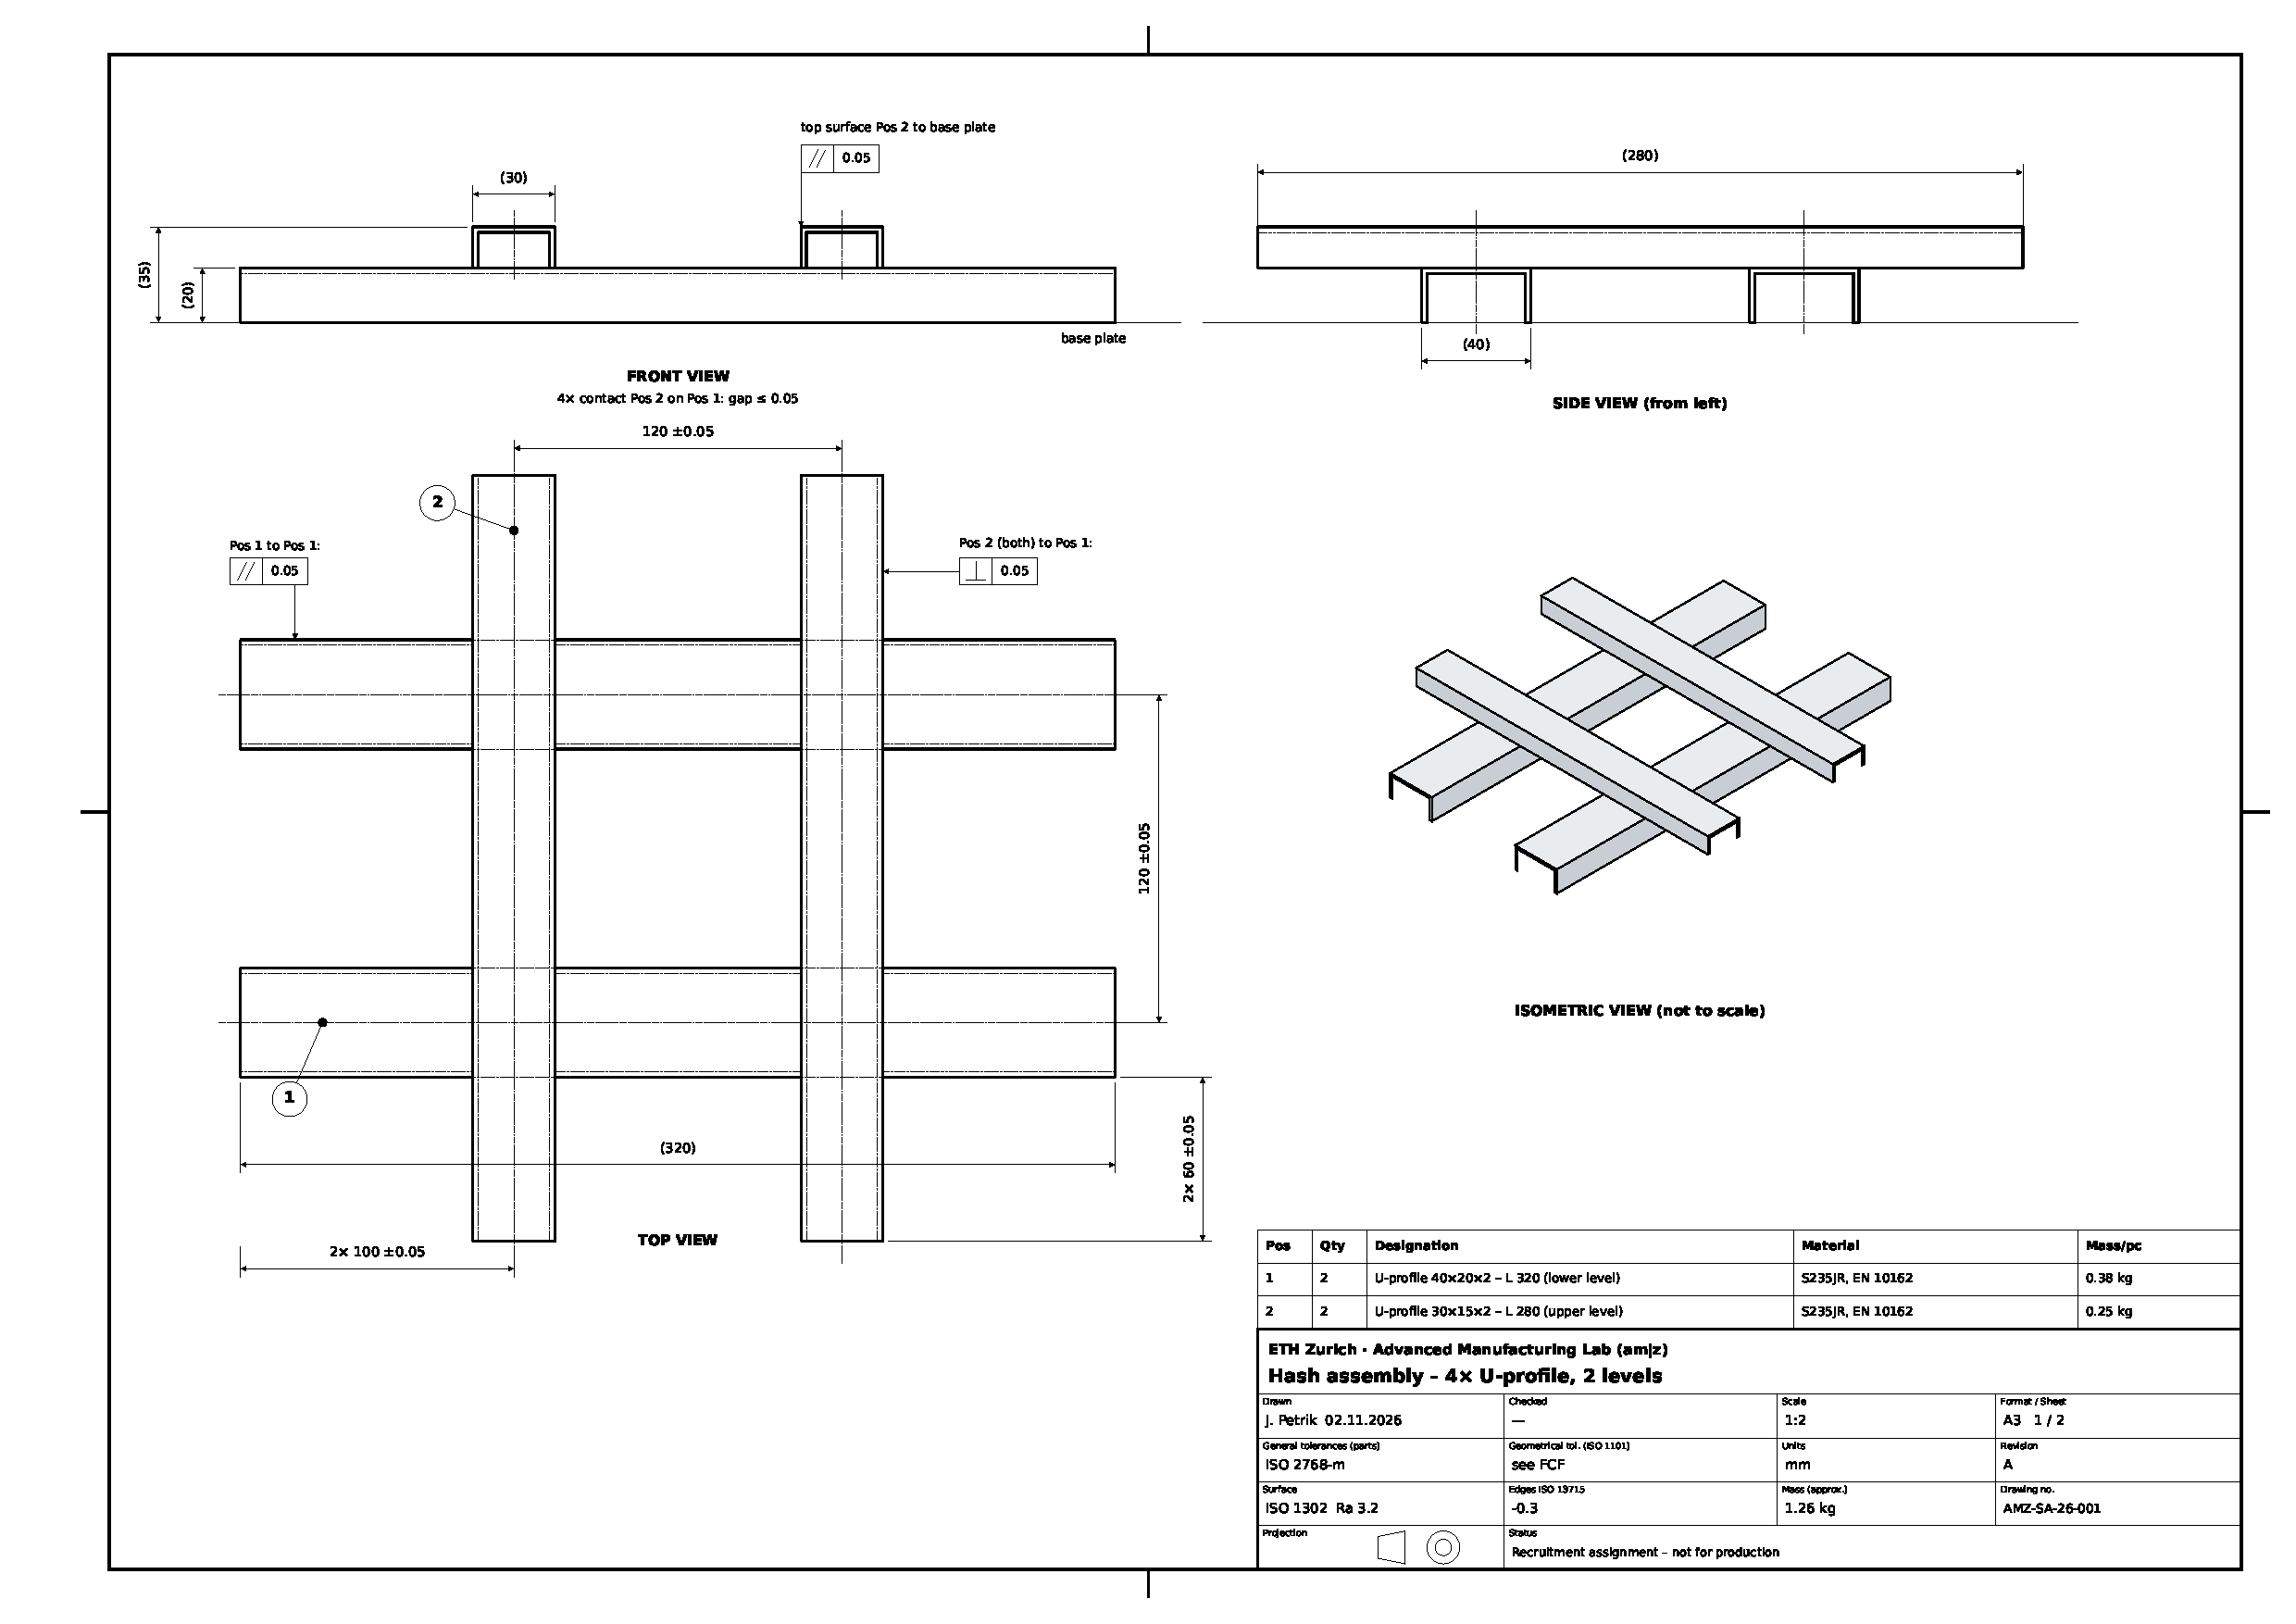
\includegraphics[angle=90,height=0.9\textheight,page=1]{figures/AMZ-SA-26-001_drawing.pdf}
\caption{Drawing AMZ-SA-26-001 rev.\ A, sheet 1/2: hash assembly (front, side, top and isometric
views) with the assembly tolerances.}
\label{fig:drawing}
\end{figure}

\begin{figure}[H]
\centering
\includegraphics[width=\textwidth,page=2]{figures/AMZ-SA-26-001_drawing.pdf}
\caption{Drawing AMZ-SA-26-001 rev.\ A, sheet 2/2: parts Pos~1 and Pos~2.}
\label{fig:drawing-parts}
\end{figure}

\begin{table}[H]
\centering
\caption{Assembly requirements from drawing AMZ-SA-26-001.}
\label{tab:req}
\begin{tabularx}{\textwidth}{@{}l L l@{}}
\toprule
ID & Characteristic & Tolerance\\
\midrule
A1 & Centre distance Pos~2 -- Pos~2 & $120\pm0.05$\,mm\\
A2 & Centre distance Pos~1 -- Pos~1 & $120\pm0.05$\,mm\\
A3 & Pos~2 axis from each end of Pos~1 & $2\times100\pm0.05$\,mm\\
A4 & Pos~2 end from the outer edge of Pos~1 & $2\times60\pm0.05$\,mm\\
A5 & Parallelism Pos~1 to Pos~1 & 0.05\,mm\\
A6 & Perpendicularity of both Pos~2 to Pos~1 & 0.05\,mm\\
A7 & Parallelism of the Pos~2 top surface to the base plate & 0.05\,mm\\
A8 & Gap at the four Pos~2 / Pos~1 contacts & $\le0.05$\,mm\\
\bottomrule
\end{tabularx}
\end{table}

Four observations shape the solution:
\begin{enumerate}
  \item \textbf{Closed chain on Pos~1:}\\ $100 + 120 + 100 = 320$. With the Pos~2 axes in place,
        the two A3 dimensions absorb the whole length error of Pos~1. Even with perfect
        positioning, A3 can only be met if the length is within $\pm0.1$\,mm (self-centring,
        error split over both ends) or $\pm0.05$\,mm (one-sided end stop). ISO 2768-m allows
        $\pm0.5$\,mm, so a conforming part can make the drawing unachievable.
  \item \textbf{Closed chain on Pos~2:}\\ $60 + 20 + 120 + 20 + 60 = 280$. A4 is referenced on the
        outer edge of Pos~1, so it carries half the Pos~1 width error ($\pm0.15$\,mm) on top of
        the Pos~2 length error.
  \item \textbf{Height stack and over-constraint:}\\ Each Pos~2 rests on two Pos~1 of height
        $20\pm0.2$\,mm. A height difference of 0.1\,mm over the 120\,mm span tilts the Pos~2 top
        by 0.23\,mm over its 280\,mm length, nearly five times the A7 zone. The four contacts on a
        $2\times2$ grid are statically indeterminate: A8 can only be met under a defined clamping
        force.
  \item \textbf{No named datums:}\\ The feature control frames refer to ``Pos~1'' without saying
        which one or which face. This report assumes datum A = base plate, B = outer side face of
        one Pos~1, C = its end face.
\end{enumerate}

In the technical drawing, the assembly appears to be simply stacked; however, to ensure that tolerances are maintained once it has been removed from the jig, the components would, for example, need to be welded together at the point of contact.

%==============================================================================
\section{The xArm6: capabilities, limits and singularities}
\label{sec:robot}

The xArm6 is well suited to transport the parts, and poorly suited to position them to a
hundredth of a millimetre. This section gives the data the cell design and the tolerance
strategy rely on.

\subsection{Specifications}

\begin{table}[H]
\centering
\caption{UFACTORY xArm6 specifications (manufacturer data).}
\label{tab:xarm}
\begin{tabularx}{\textwidth}{@{}l L@{}}
\toprule
Degrees of freedom & 6, all revolute\\
Payload & 5\,kg\\
Reach & 700\,mm\\
Repeatability & $\pm0.1$\,mm\\
Absolute accuracy & not published\\
Max TCP speed / joint speed & 1\,m/s / $180^\circ$/s\\
Joint ranges & J1 $\pm360^\circ$; J2 $-117^\circ$ to $116^\circ$; J3 $-219^\circ$ to $10^\circ$;
J4 $\pm360^\circ$; J5 $-97^\circ$ to $180^\circ$; J6 $\pm360^\circ$\\
Arm mass, footprint, mounting & 12.5\,kg, \O126\,mm, any orientation\\
Structure & aluminium and carbon fibre links, harmonic drives, BLDC motors\\
Tool flange & ISO 9409-1-50-4-M6 (\O50\,mm pitch circle, 4$\times$M6, dowel pin)\\
Power & 24\,V DC, typically 200\,W\\
Interfaces & Ethernet (proprietary TCP protocol), Modbus TCP to the tool, 16 digital in/out,
2 analog in/out, RS-485\\
Programming & UFACTORY Studio, Python and C++ SDK, ROS/ROS~2\\
\bottomrule
\end{tabularx}
\end{table}

\subsection{Advantages for this task}

\begin{itemize}
  \item \textbf{Payload and reach margins:}\\ The heaviest part is 0.38\,kg, so even with a 1\,kg
        gripper the arm works at a quarter of its rated payload. With the tool vertical at
        placing height, the horizontal reach found by inverse kinematics is 712\,mm; the farthest
        corner of the fixture is 680\,mm from each base.
  \item \textbf{Open software:}\\ The Python SDK and ROS~2 packages allow the same task code to run
        in simulation and on the arms, and give access to joint-level streaming, which closed
        teach-pendant languages do not.
  \item \textbf{Collaborative and light:}\\ Collision detection, 12.5\,kg arm, any mounting, a
        6-axis force/torque sensor option for force-controlled insertion against fixture datums.
  \item \textbf{Cost:}\\ About EUR~11\,000 per arm, which makes a two-arm research cell affordable.
\end{itemize}

\subsection{Particularities and weaknesses}

\begin{itemize}
  \item \textbf{Repeatability versus accuracy:}\\ $\pm0.1$\,mm repeatability is twice the assembly
        tolerance. Absolute accuracy, which matters for a fixture located by coordinates, is not
        published; for an uncalibrated arm of this class it is expected at the millimetre level.
        This report assumes $\pm1$\,mm and plans to measure it (Section~\ref{sec:valid}).
  \item \textbf{Error amplification:}\\ At the cycle poses, an error of only $0.01^\circ$ on every
        joint moves the TCP by up to 0.27--0.30\,mm (Table~\ref{tab:poses}): encoder resolution,
        harmonic-drive backlash and the compliance of light links are enough to exceed the
        tolerance.
  \item \textbf{Compliance and thermal drift:}\\ Carbon links and harmonic drives are light but less
        stiff than a cast industrial arm; the deflection depends on the payload and the pose,
        and warm-up shifts the TCP.
  \item \textbf{Offset wrist:}\\ The links carry lateral offsets (53.5\,mm and 77.5\,mm in the
        upper arm and forearm), and the wrist is not spherical: with J5 at zero, the J4 and J6
        axes are parallel but 76\,mm apart. Position and orientation are therefore coupled, the
        inverse kinematics has no simple closed form, and the singular configurations are
        surfaces that depend on several joints.
  \item \textbf{Two independent controllers:}\\ Each arm has its own controller and there is no
        native synchronised dual-arm mode; coordination is done in our software (zone lock,
        precedence) and the two base frames must be calibrated against each other.
\end{itemize}

\subsection{Singularities}

Near a singularity a small TCP motion requires large joint speeds and the arm loses
stiffness in some directions; the UFACTORY manual asks to avoid moving the wrist close to the
cylinder above and below the base. Three families matter for this cell, all checked on the
model built from the official \code{xarm\_ros2} kinematics:
\begin{itemize}
  \item \textbf{Elbow:}\\ upper arm and forearm aligned, at J3 $\approx-157^\circ$ given the link
        offsets; this is the boundary of the reach.
  \item \textbf{Shoulder:}\\ the wrist centre on the J1 axis, directly above the base.
  \item \textbf{Wrist alignment:}\\ J5 $\to0$, J4 parallel to J6. With the tool vertical this
        happens on a ring about 300\,mm from the base (Figure~\ref{fig:dex}).
\end{itemize}

The dexterity is measured by the inverse condition number of the Jacobian (rows mixed with a
characteristic length of 0.3\,m): 1 for an isotropic pose, 0 at a singularity.
Figure~\ref{fig:dex} maps it for robot~A with the tool vertical at placing height. The first
layout placed the magazines 300\,mm from the base, right on the low-dexterity ring: the pick
poses had J5 at $3.4^\circ$ and an inverse condition number of 0.016. Moving the magazines to
450\,mm raised it to 0.081 (J5 at $19^\circ$). Table~\ref{tab:poses} gives the margins of the
final poses; robot~B is the mirror image of robot~A.

\begin{figure}[H]
\centering
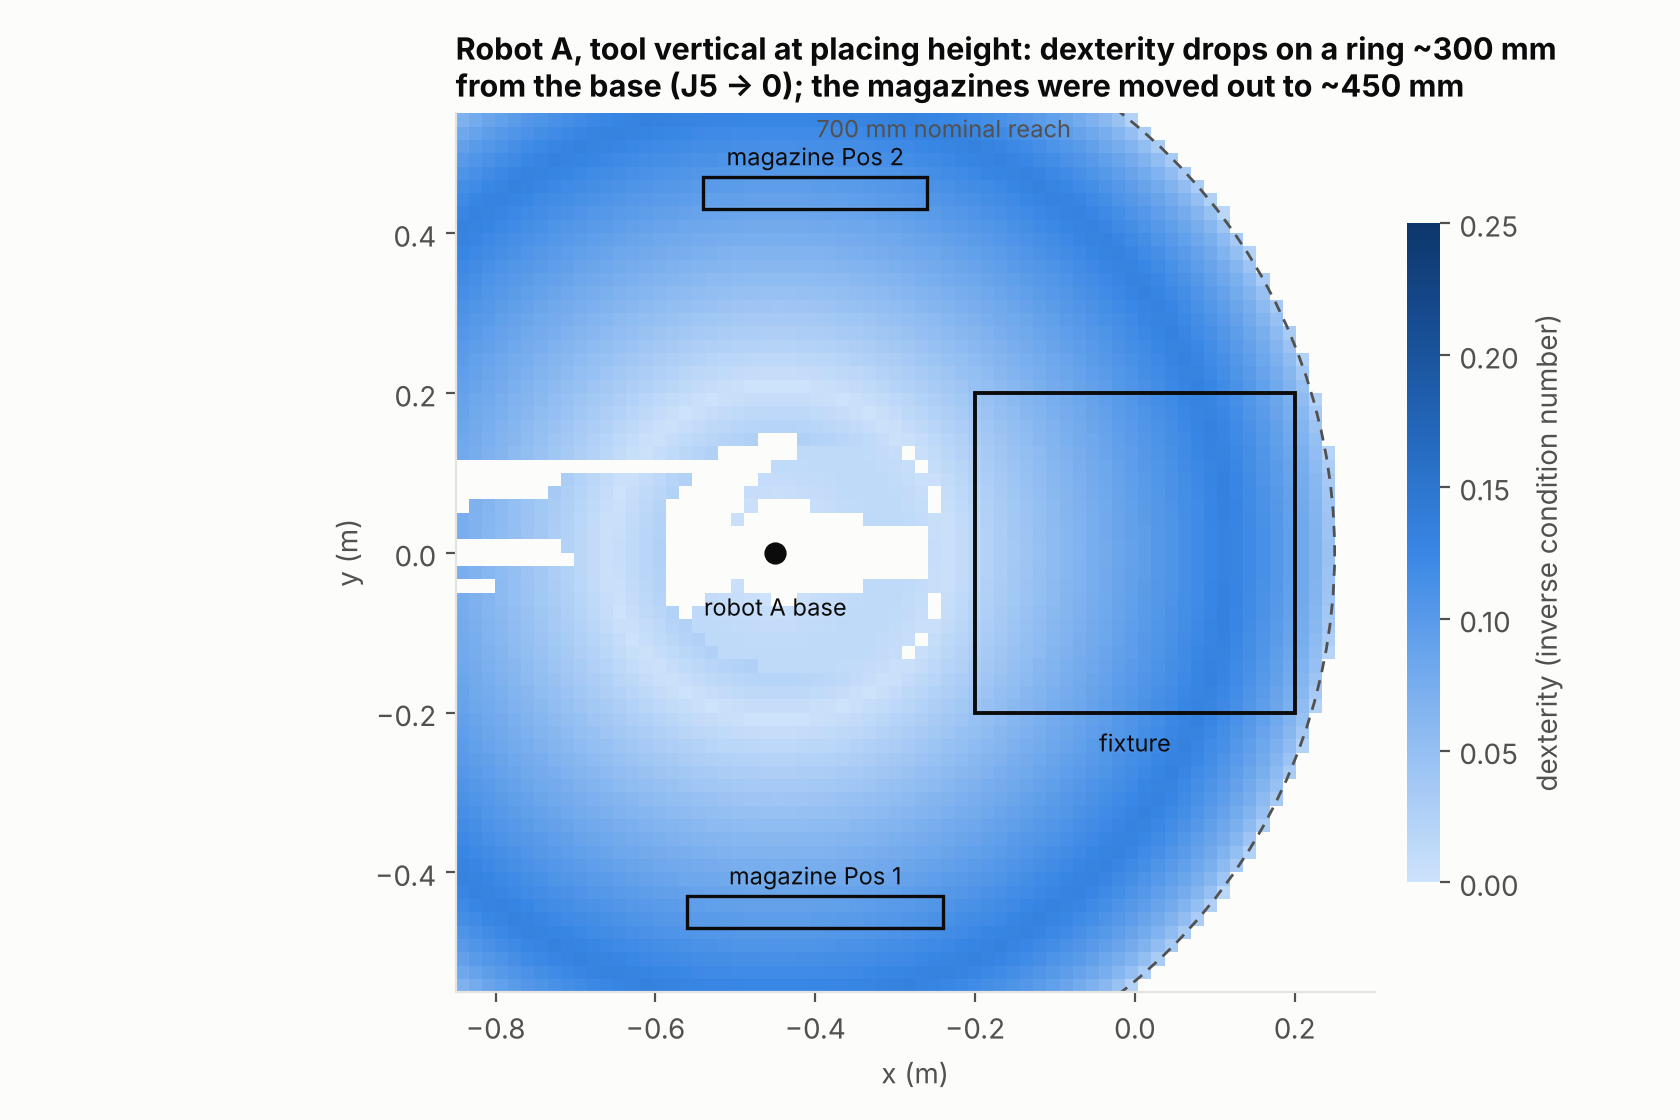
\includegraphics[width=0.85\textwidth]{figures/fig_xarm6_dexterity.png}
\caption{Dexterity of robot~A, tool vertical at placing height. White: no solution found with
the tool vertical, close to the base (shoulder zone) and beyond the reach.}
\label{fig:dex}
\end{figure}

\begin{table}[H]
\centering
\caption{Distance of the cycle poses of robot~A to the singularities, and TCP error for
$0.01^\circ$ on every joint (worst case).}
\label{tab:poses}
\small
\begin{tabular}{@{}lrrrrr@{}}
\toprule
Pose of robot A & Dexterity & J5 & Elbow & Wrist to & TCP\\
 & & & margin & J1 axis & error\\
\midrule
Pick, magazine at 300\,mm (first layout) & 0.016 & $3.4^\circ$ & $137^\circ$ & 228\,mm & 0.26\,mm\\
Pick, magazine at 450\,mm & 0.081 & $19.4^\circ$ & $107^\circ$ & 377\,mm & 0.30\,mm\\
Place Pos~1 & 0.092 & $22.1^\circ$ & $107^\circ$ & 378\,mm & 0.30\,mm\\
Place Pos~2 & 0.083 & $19.1^\circ$ & $122^\circ$ & 314\,mm & 0.28\,mm\\
100\,mm above the fixture & 0.14 & $34^\circ$ & $108^\circ$ & 378\,mm & 0.29\,mm\\
\bottomrule
\end{tabular}
\end{table}

\subsection{Built-in collision detection}

Without joint torque sensors, the controller detects collisions from the motor currents
(sensitivity 0--5).\footnote{UFACTORY, \emph{Collision detection in UFACTORY robotic arms:
		current and dynamic model-based feature}, support article.} It reacts only after contact and
ignores the other arm, so it does not replace the zone lock (Section~\ref{sec:coord}). On the
real cell it is a secondary safety layer: payload updated at each grasp, lower sensitivity
during insertion, rebound disabled. It is not modelled in MuJoCo.

\textbf{Consequences for the design:} 

The robot moves parts to within a few millimetres, in
well-conditioned poses; everything below a millimetre is left to the fixture
(Section~\ref{sec:tol}).\\

%==============================================================================
\section{Cell design}

The two robots face each other, with the fixture in the centre. On either side of the robots are the profiles to be positioned. The space shared by the two robots is therefore limited to the central area only (Figure~\ref{fig:cell}). There is no limit on the payload, as a profile weighs a maximum of 0.38\,kg, whilst the robot can lift 5\,kg
\begin{figure}[H]
\centering
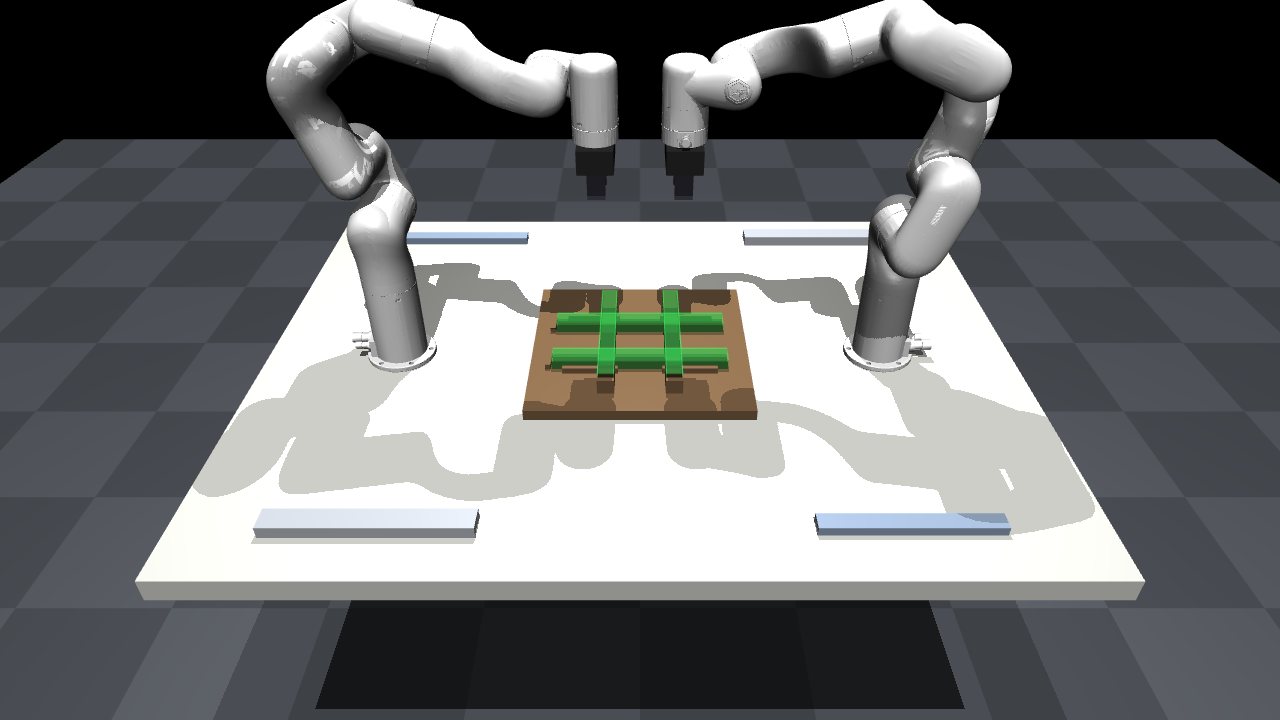
\includegraphics[width=0.85\textwidth]{figures/scene_overview.png}
\caption{Simulated cell (MuJoCo). The green transparent profiles are the nominal assembled
positions; the four loose profiles lie in their magazines.}
\label{fig:cell}
\end{figure}

\textbf{Layout:} 

The robots are mounted on a rigid table measuring $1.4\times1.1$\,m at $x=\pm0.45$\,m from the
fixture centre.
Robot~A serves the Pos~1 and Pos~2 on its side ($y<0$ and $x<0$), whilst robot~B serves the symmetrical positions, enabling both robots to operate simultaneously.. Furthermore, all pick-up and set-down positions are accessible with the tool in a vertical position; this has been verified by an automated test for both robots, at the pick-up height and 80\,mm above it.

\textbf{Magazines:} 

Parts arrive flanges down in nested trays or gravity magazines with known
orientation ($\pm2$\,mm, $\pm2^\circ$). Pos~1 and Pos~2 have different tray shapes, which
prevents mixing them up. The magazines sit 450\,mm from their robot base, outside the
low-dexterity ring identified in Section~\ref{sec:robot}.

\textbf{Gripper:} 

An electric parallel gripper with long, 30\,mm wide pads grips the two
flanges from outside; the choice is argued in Section~\ref{sec:gripper}.

\textbf{Fixture (the precision element):}

A machined plate, flat to $\le0.01$\,mm, which is also
the base plate of the drawing, carries every reference:
\begin{itemize}
  \item for each Pos~1, two grooves at 120\,mm with lead-in chamfers giving a capture range of at
        least $\pm2$\,mm, a side reference (datum B) and an end stop (datum C);
  \item relief pockets in the side references where the gripper fingers go down: in a first
        simulation a finger, 8\,mm thick, hit the rail on release and dragged the part by
        8\,mm;
  \item for each Pos~2, overhanging guides at 120\,mm, perpendicular to the Pos~1 grooves;
  \item self-centring jaws (pneumatic) that centre each part in length and width, so that
        dimension errors split equally between both sides;
  \item four clamps at the crossings that close the A8 gaps before joining, with access left for
        the welding torch or adhesive nozzle and for measurement.
\end{itemize}

In the present simulation the fixture is passive: plate, side rails with finger pockets and
end stops, with a 1.5\,mm lead-in clearance. The active jaws and clamps are not simulated; their effect is
quantified by the tolerance model in Section~\ref{sec:tol}.

\subsection{Why this gripper}
\label{sec:gripper}

The gripper must pick both profiles without a tool change, hold them during the transfer and
release them without moving them. Since the parts lie flanges down, only two surfaces are
accessible: the flat web on top (30 or 40\,mm wide) and the outer faces of the two flanges
(15 or 20\,mm high).

\begin{table}[H]
\centering
\caption{Gripper options for the U-profiles.}
\label{tab:gripper}
\small
\begin{tabularx}{\textwidth}{@{}p{2.9cm} L L@{}}
\toprule
Option & For & Against\\
\midrule
\textbf{Electric parallel gripper} on the outer flanges (e.g.\ UFACTORY Gripper G2: 84\,mm stroke,
10--50\,N, 800\,g) &
both widths (30, 40\,mm) with one stroke; centres the part in width; force and position
controlled and read back; plugs into the xArm tool port (Modbus RTU); no air supply &
fingers occupy the outer faces, which are also the side datums of the fixture (needs relief
pockets); grips the 2\,mm flanges, so closing must be slow and force-limited\\
Vacuum cup on the web & simplest; no finger clearance needed in the fixture; cheap &
no centring; the part can slip or turn on the cup during accelerations (320\,mm long part held at
one point); needs a pump or compressed air\\
Magnetic gripper (steel parts) & strong hold, no contact with the datum faces &
no centring; the 2\,mm web limits the holding force; residual magnetism and slow, imprecise
release; attracts chips, can disturb sensors\\
\bottomrule
\end{tabularx}
\end{table}

\textbf{Choice, electric parallel gripper with custom fingers:}

It is the only option that centres the part in width while carrying it, which reduces the error
left to the fixture. It also releases the part simply by opening, without suction loss or
residual magnetism. The fingers are designed as follows:
\begin{itemize}
  \item \textbf{Width:}\\ 30\,mm pads, so that a 320\,mm part held at its middle does not pivot.
  \item \textbf{Length:}\\ the fingers reach 1\,mm above the bottom of the flanges, to grip the
        part as low as possible.
  \item \textbf{Facing:}\\ polyurethane ($\mu\approx0.5$, assumed). With $F=20$\,N per finger, the
        holding force $2\mu F$ is 20\,N, against 7.5\,N needed for a 0.38\,kg part accelerated at
        1\,g. With bare steel ($\mu\approx0.2$), almost no margin would be left.
  \item \textbf{Thickness:}\\ 8\,mm, so that the fingers fit into the relief pockets of the fixture
        rails.
\end{itemize}

The gripper closes slowly, with a force limit of 20\,N per finger (within the G2 range). These
settings come from two problems seen in simulation: a fast closure made a finger pass through the
2\,mm flange, and a finger that hit a rail on release dragged the part by 8\,mm. A compliant mount
between the robot flange and the gripper would also help the part follow the lead-in chamfers.

In simulation, the gripper is a generic model: its opening (50\,mm) and force are within the G2
ranges, but its mass and closing speed are not those of the real gripper. Only the fingers, which
touch the part, have their real dimensions. On the real cell, the gripper is mounted on the tool
flange (ISO~9409-1-50-4-M6) with a dowel pin, so that the TCP is reproducible; it is still checked
after each remounting.

%==============================================================================
\section{Assembly sequence and dual-arm coordination}
\label{sec:coord}

The robots take turns: one picks and places its part while the other waits above its next part.
A Pos~2 is placed only once both Pos~1 are in the fixture.
\begin{enumerate}
  \item A and B move above their Pos~1, gripper open.
  \item A enters the fixture zone, picks and places its Pos~1, then waits above its Pos~2. B
        waits.
  \item B enters the zone, picks and places its Pos~1. A waits.
  \item With both Pos~1 in place, A then B place their Pos~2 across them.
  \item On the real cell, the fixture then centres the Pos~2 and clamps the four crossings; the
        assembly is measured, joined, unclamped and unloaded.
\end{enumerate}

Two rules coordinate the robots:
\begin{itemize}
  \item \textbf{Zone lock:}\\ only one robot at a time in the fixture zone. The other waits above
        its magazine until the zone is free. This prevents any collision between the arms without
        having to plan the motion of both arms together (12 axes).
  \item \textbf{Precedence:}\\ a Pos~2 is placed only after both Pos~1.
\end{itemize}

A robot grips its part only once it has access to the zone, so it never waits with a part in the
gripper. In a first version, the robots picked first and then waited: during a 5\,s wait, a part
slid out of the simulated gripper. This change costs a few seconds per cycle but avoids dropping a
part during a stop.

\textbf{Measured grasp:}

Before placing a part, the robot checks where the part actually is in the gripper, and positions
the part rather than the TCP. In simulation, the part slides by 2--4\,mm in the gripper during the
transfer; without this check, it landed on the edge of a rail. On the real cell, a camera or a
laser sensor would make this measurement.

The simulation gives a cycle time of 32\,s for one assembly (Figure~\ref{fig:timeline}). The
fixture zone is the bottleneck. The cycle could be shortened by letting A and B place their Pos~1
at the same time from opposite sides, or by gripping the next part while the other robot leaves
the zone.

\begin{figure}[H]
\centering
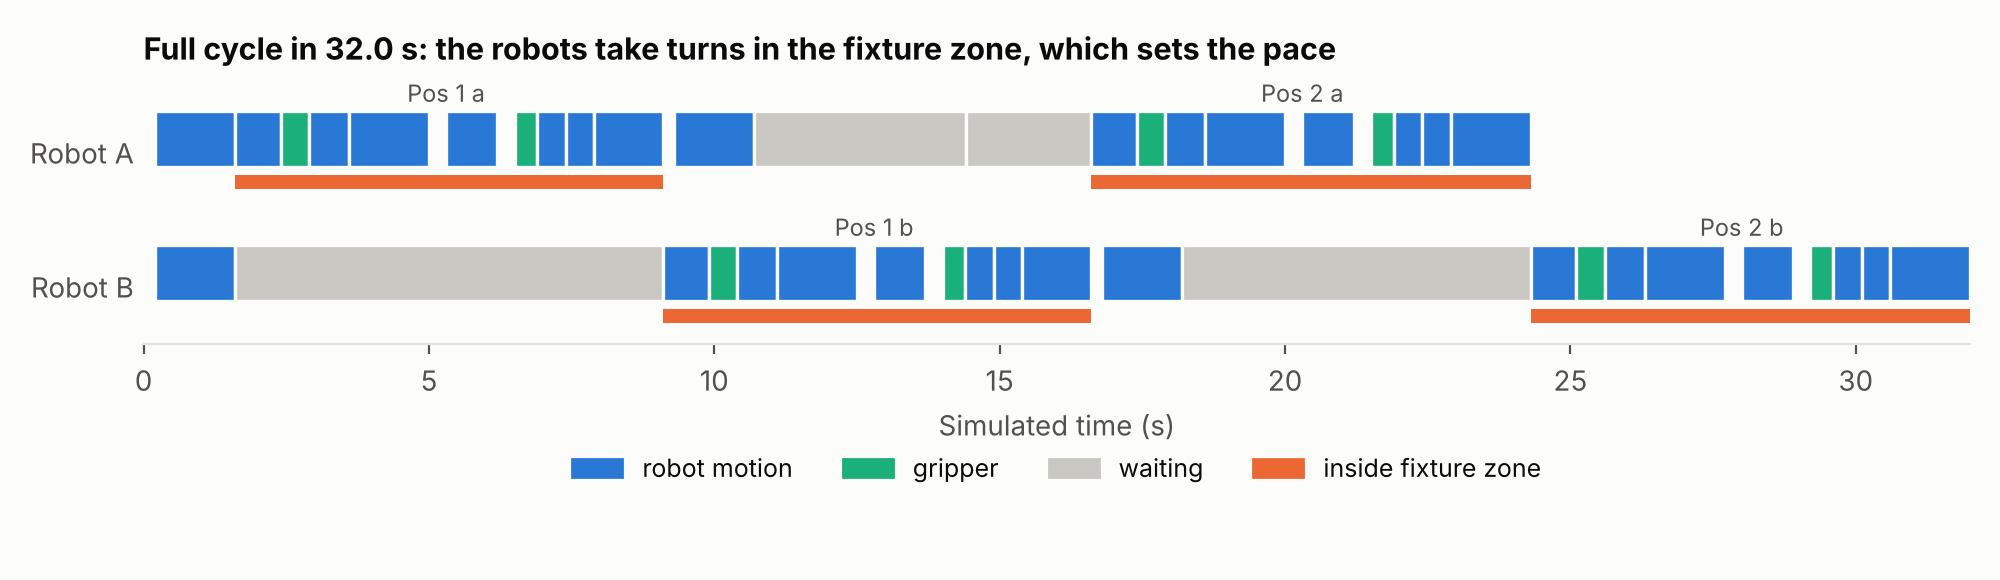
\includegraphics[width=\textwidth]{figures/fig_cycle_timeline.png}
\caption{Timeline of one simulated cycle. Orange bars: robot holding the fixture-zone lock, from
the pick to the exit of the zone; the bars never overlap.}
\label{fig:timeline}
\end{figure}

%==============================================================================
\section{Software architecture}

The code is written in Python with the MuJoCo physics engine. A generic \code{Robot} interface
separates the cycle logic from the simulator, so that the same logic can later drive the real
robots through the xArm Python SDK (Section~\ref{sec:sim2real}).

\subsection{Why MuJoCo}

The simulation had to answer four questions: can both robots reach every pose, does the two-robot
sequence run without collision, how does a part behave when it is released into the fixture, and
how large is the placement error. The last two depend on contacts between thin steel parts,
fingers and fixture, so contact quality mattered more than graphics or ROS integration.

\begin{table}[H]
\centering
\caption{Simulation tools considered.}
\label{tab:sim}
\small
\begin{tabularx}{\textwidth}{@{}p{2.8cm} L L@{}}
\toprule
Tool & Strength & Why not chosen here\\
\midrule
\textbf{MuJoCo} (chosen) & fast, stable rigid contacts with friction; direct Python access to
the full state, contact forces and Jacobians; deterministic and headless, so it runs in pytest
and in batches (31 full cycles in about a minute); installs with \code{pip} on Windows and Linux &
no ready-made xArm6 model (only xArm7 and Lite~6 in MuJoCo Menagerie), so the model was built from
the official kinematics\\
Gazebo + ROS~2 + MoveIt~2 & UFACTORY ships Gazebo and MoveIt configurations; closest to a ROS
deployment & heavier set-up (Linux, ROS distribution, controllers), slower iteration; contacts of
thin parts less reliable; kept as a deployment option\\
PyBullet & similar ease of use in Python & fewer contact-solver options (cone type, implicit
integration); no advantage for this task\\
NVIDIA Isaac Sim & photorealistic sensors (cameras), GPU parallelism & needs an RTX GPU and a heavy
installation; out of proportion for four parts\\
RoboDK, ABB RobotStudio & offline programming, reach and cycle-time studies & no contact physics;
RobotStudio's virtual controller is for ABB robots only\\
\bottomrule
\end{tabularx}
\end{table}

I had already used MuJoCo for my Master's thesis (whole-body control of the 32-DOF TALOS
humanoid), which made the set-up faster.

\textbf{Limits met during the work:}

MuJoCo contacts are slightly soft: parts sink by about 0.02\,mm, a part held for several seconds
slid out of the gripper, and a fast closure made a finger pass through a 2\,mm flange. Each problem
was solved (slow closure with a force limit, gripping only when needed). The robot model is also
ideal: no backlash, no deformation, no calibration error. The simulation is therefore used to check
the logic (reach, sequence, coordination, capture by the fixture), and accuracy is studied with the
tolerance model (Section~\ref{sec:tol}).

\subsection{Code structure and tests}

\begin{table}[H]
\centering
\caption{Repository structure.}
\begin{tabularx}{\textwidth}{@{}l L@{}}
\toprule
Module & Role\\
\midrule
\code{config/cell.yaml} & every cell parameter: robot bases, gripper, fixture, parts, magazines\\
\code{scene.py} & generates the MuJoCo model from the config; xArm6 kinematics, joint limits and
link inertias taken from the official \code{xarm\_ros2} description\\
\code{ik.py} & damped least-squares inverse kinematics; for the symmetric gripper it tries both
equivalent grasps ($180^\circ$ about the tool axis) and keeps the one closest to the current
posture\\
\code{cycle.py} & robot programs as Python generators advanced once per simulation step (true
concurrency), zone lock, precedence, event log\\
\code{tolerance/} & tolerance chains of A1--A8 and the Monte-Carlo; every assumed input is listed
in \code{params.py}\\
\code{analyze\_xarm6.py} & singularity margins of the cycle poses, dexterity map, error
amplification\\
\code{robot\_interface.py}, \code{backends/} & hardware abstraction; MuJoCo backend implemented,
xArm SDK backend to be added\\
\bottomrule
\end{tabularx}
\end{table}

\textbf{Testing and CI:}

15 tests run automatically with GitHub Actions at each push. They check that:
\begin{itemize}
  \item the scene loads and is stable;
  \item both robots reach every pick and place pose;
  \item the full cycle completes without breaking the zone lock or the precedence;
  \item the tolerance model gives the same results as the hand calculations.
\end{itemize}

\textbf{Run it:}

\code{pip install -r requirements.txt}, then \code{python scripts/run\_cycle.py --viewer} (cycle),
\code{python scripts/run\_montecarlo.py} (tolerance analysis) and \code{python -m pytest} (tests).

%==============================================================================
\section{Simulation results}

The cycle works, but the robot alone places the parts with an error of about one millimetre, some
twenty times the $\pm0.05$\,mm tolerance.

\textbf{Full cycle:}

The four parts are picked, transferred and placed in 32\,s, without collision between the arms.
The height error is 0.02\,mm, which is the contact penetration of the simulator. The cycle is shown
in the video \code{docs/cycle.mp4}.

\textbf{Free placement:}

The cycle was run with an ideal robot, then with a robot error of $\pm1$\,mm ($3\sigma$) added at
each placement. This value is an assumption for the absolute accuracy of this type of robot; the
$\pm0.1$\,mm of the datasheet is only the repeatability.

\begin{table}[H]
\centering
\caption{Free placement: final planar error of the parts released by the robot alone.}
\begin{tabular}{@{}lrrrr@{}}
\toprule
Robot error at the fixture & Parts & Mean error & Max error & Within $\pm0.05$\,mm\\
\midrule
none (ideal robot) & 4 & 0.67\,mm & 1.15\,mm & 0\,\%\\
$\pm1$\,mm ($3\sigma$) & 120 (30 cycles) & 0.66\,mm & 1.55\,mm & 1\,\%\\
\bottomrule
\end{tabular}
\end{table}

Even an ideal robot misses by up to 1.2\,mm, because the part moves when it is released and when it
touches the fixture. With the $\pm1$\,mm error, the result hardly changes: the passive rails and
stops keep each part within their 1.5\,mm lead-in clearance, so the fixture already absorbs the
robot error. In earlier runs, before the finger relief pockets were added, a finger caught on a rail
and the error reached 7\,mm. A Pos~2 placed off target could also push a Pos~1 sideways, so each
part must be clamped before the next one is placed on it.

To go from 1\,mm to 0.05\,mm, the fixture must actively centre and clamp the parts: the accuracy
comes from what happens after the release, not from the robot trajectory.

\begin{figure}[H]
\centering
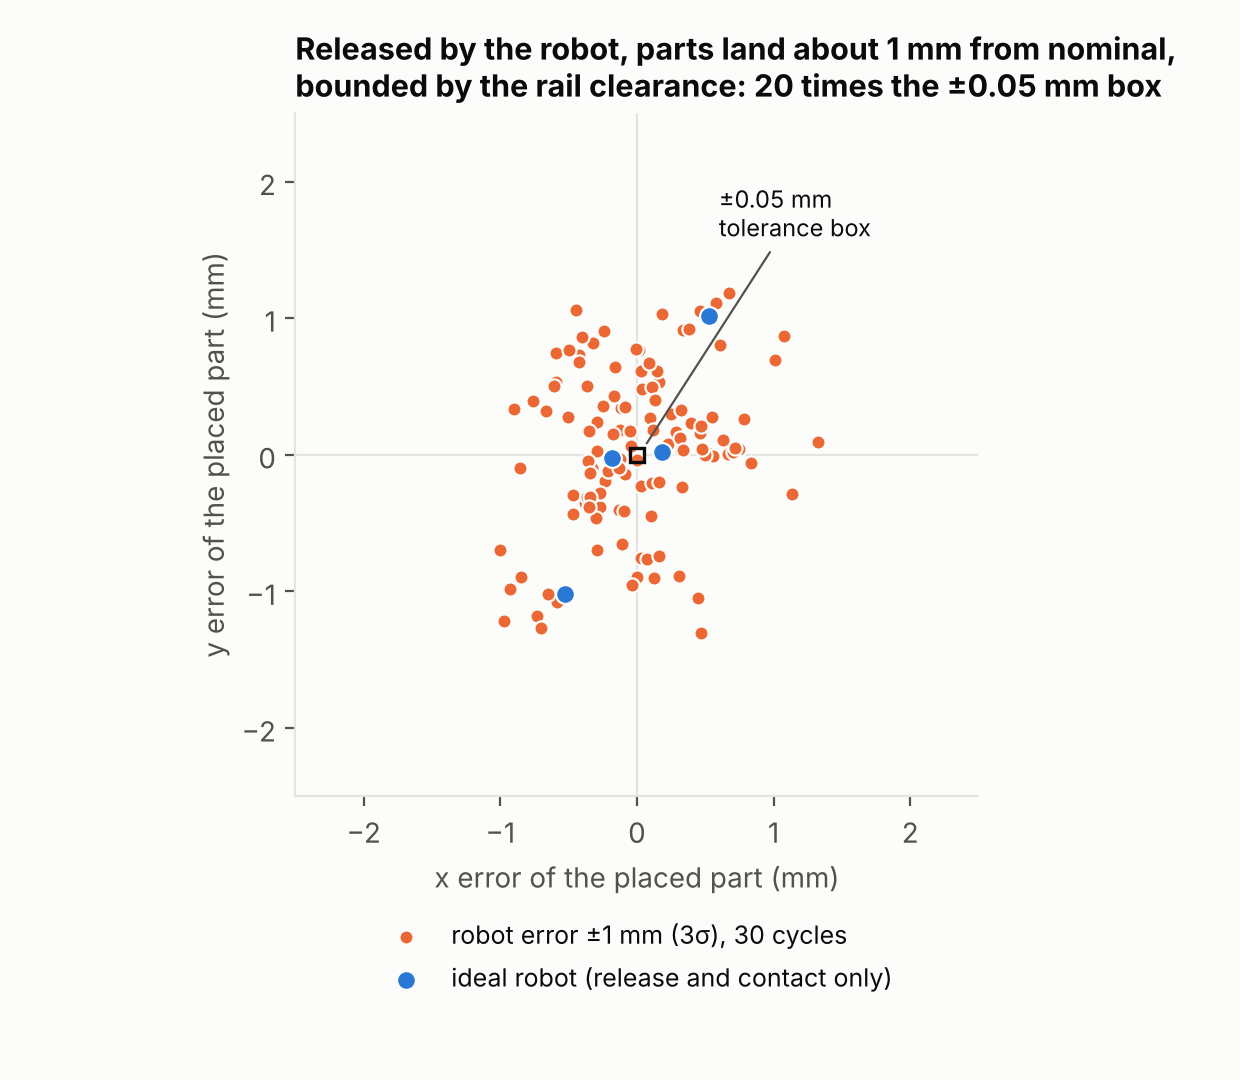
\includegraphics[width=0.6\textwidth]{figures/fig_free_placement.png}
\caption{Final position error of each part released by the robot alone, ideal robot and
$\pm1$\,mm robot. The $\pm0.05$\,mm tolerance box is the small square at the origin.}
\label{fig:free}
\end{figure}

%==============================================================================
\section{Meeting the tolerances (reality check)}
\label{sec:tol}

Each tolerance is assigned to an element that is more accurate than the tolerance itself, never to
the robot. When the parts themselves make a tolerance impossible, the parts are controlled or the
assembly is machined after joining.

\subsection{Strategy per requirement}

\begin{table}[H]
\centering
\caption{Which element holds each requirement.}
\begin{tabularx}{\textwidth}{@{}p{3.3cm} L L@{}}
\toprule
Requirement & Dominant error source & What holds it\\
\midrule
A1, A2 centre distances & robot position ($\pm1$\,mm), part widths & grooves machined to
$\pm0.01$\,mm; self-centring jaws make the axis independent of the width\\
A5, A6 parallelism, perpendicularity & robot orientation, part bow & fixture reference faces;
part clamped along its length\\
A3 $2\times100$ & Pos~1 length ($\pm0.5$\,mm) & closed chain: length control or end machining
(\ref{sec:parts})\\
A4 $2\times60$ & Pos~2 length, Pos~1 width ($\pm0.3$\,mm) & end machining of Pos~2\\
A7 top parallelism & height difference of the two Pos~1 ($\pm0.2$\,mm each) & Pos~1 cut
consecutively from one bar or sorted by measured height\\
A8 gaps & over-constrained 4-point support, flange flatness & clamps at the crossings close the
gaps elastically; joining under clamping\\
all, after unclamping & spring-back & joining (tack weld or adhesive) before release\\
\bottomrule
\end{tabularx}
\end{table}

The robot only needs to bring each part within the $\pm2$\,mm capture range of the lead-in
chamfers; beyond that, its accuracy no longer matters. Calibration (TCP, fixture position, common
frame of the two robots) is only needed to stay within this range. A correction made by the robot
itself cannot be more precise than the robot's repeatability, which is why the final positioning is
done by mechanical references.

\subsection{Monte-Carlo model}

The eight characteristics are computed for 100\,000 simulated assemblies per scenario. Part
dimensions follow normal distributions (tolerance $=3\sigma$); the other errors (robot, gripper,
fixture, part shape) use the values of Section~\ref{sec:assump}.

\begin{table}[H]
\centering
\caption{Scenarios of the tolerance analysis.}
\begin{tabularx}{\textwidth}{@{}l L@{}}
\toprule
Scenario & Placement and parts\\
\midrule
S0 & robot alone, parts released at nominal coordinates\\
S1 & fixture with one-sided datum stops (end stop and side rail)\\
S2 & fixture with self-centring jaws\\
S3 & S2 + lengths cut to $\pm0.05$\,mm + Pos~1 paired by height\\
S4 & S2 + Pos~1 paired by height + ends machined after joining ($\pm0.02$\,mm)\\
\bottomrule
\end{tabularx}
\end{table}

Figure~\ref{fig:heatmap} shows the share of conforming assemblies:
\begin{itemize}
  \item The robot alone never produces a conforming assembly.
  \item The self-centring fixture secures A1, A2, A5, A6 and A8 (100\,\% in S2).
  \item One-sided stops are worse (52\,\% on A2 instead of 100\,\%), because the part width then
        shifts the part axis.
  \item A3, A4 and A7 depend on the parts, whatever the positioning: in S2, only 17\,\% of the
        assemblies meet A3 and 6\,\% meet A4.
\end{itemize}

\begin{figure}[H]
\centering
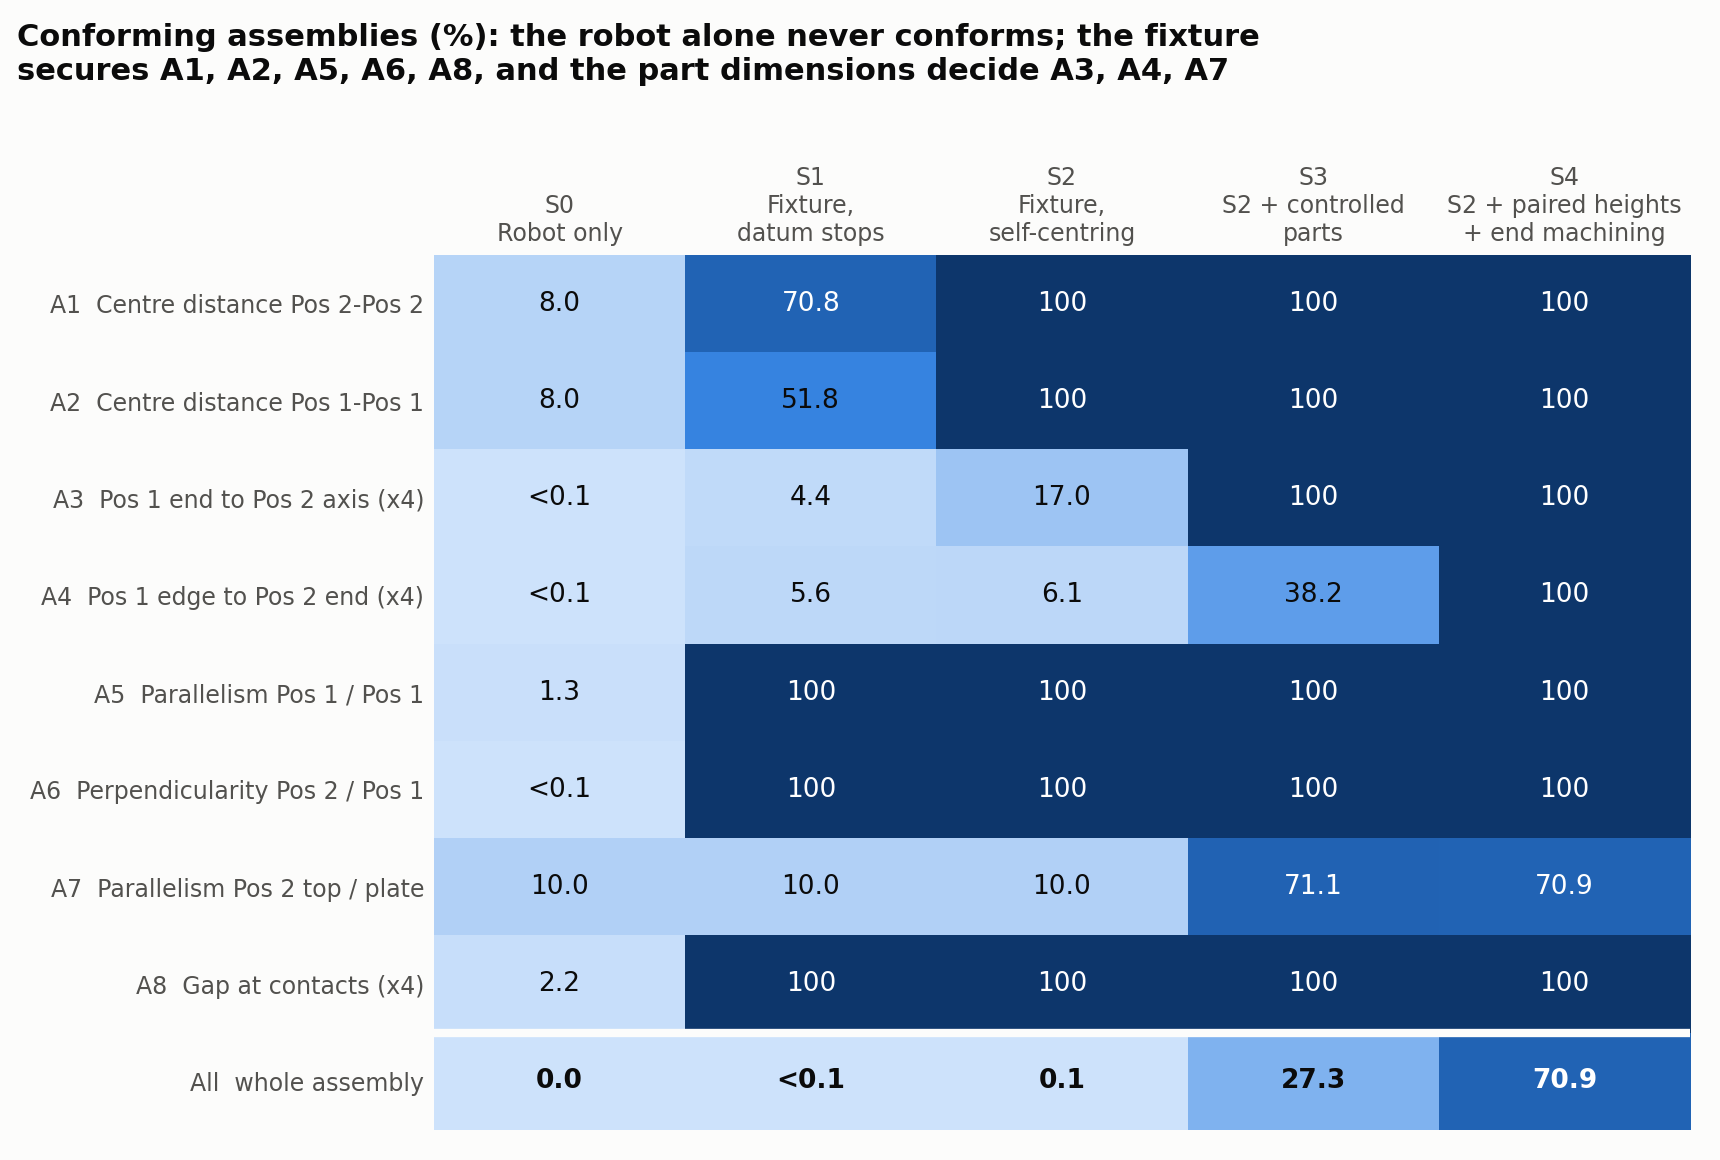
\includegraphics[width=0.92\textwidth]{figures/fig_yield_heatmap.png}
\caption{Share of conforming assemblies (\%) per characteristic and scenario, 100\,000 assemblies
each.}
\label{fig:heatmap}
\end{figure}

\begin{figure}[H]
\centering
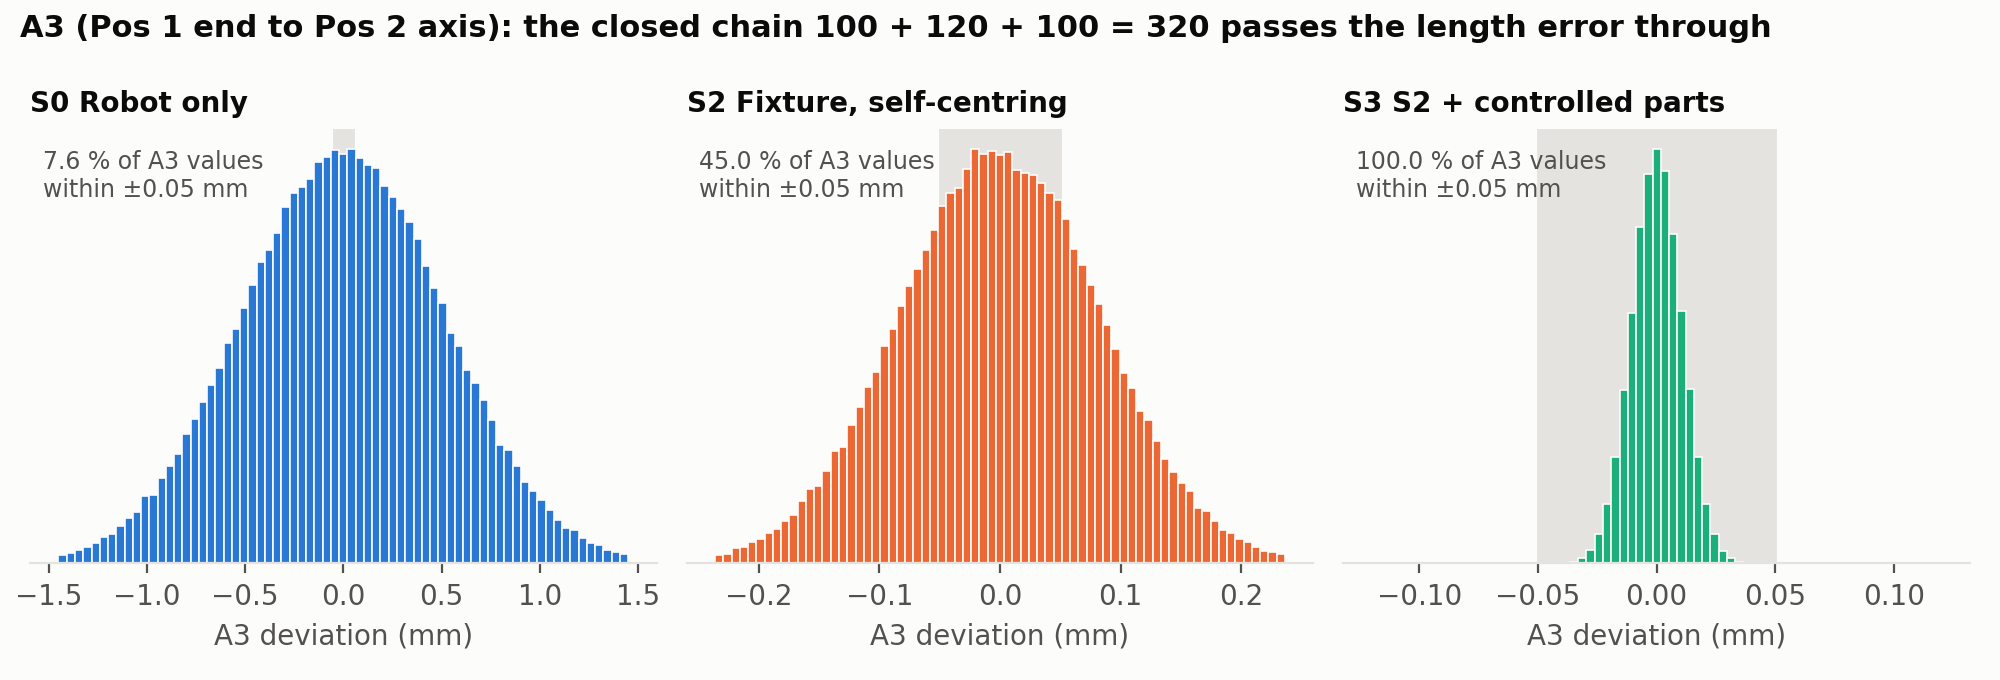
\includegraphics[width=\textwidth]{figures/fig_a3_hist.png}
\caption{Distribution of the A3 deviation in three scenarios (grey band: $\pm0.05$\,mm). The
fixture removes the robot error, but the closed chain still passes the Pos~1 length error through
until the lengths are controlled.}
\label{fig:a3}
\end{figure}

\subsection{What the part tolerances must be}
\label{sec:parts}

A3 reaches 98\,\% only if the part lengths are within $\pm0.1$\,mm (Figure~\ref{fig:cut}), five
times tighter than the drawing ($\pm0.5$\,mm, which gives 17\,\%). A4 stays below about 40\,\% even
with perfect lengths, because the width of Pos~1 ($\pm0.3$\,mm) is part of its chain. There are
three ways to solve these closed chains:
\begin{enumerate}
  \item \textbf{Precision cutting and sorting:}\\ cut the lengths to $\pm0.05$\,mm and pair the
        Pos~1 by measured height. This solves A3 but not A4 (S3: 27\,\% of assemblies fully
        conforming).
  \item \textbf{Machining the ends after joining:}\\ machine the ends, referenced on the Pos~2 axes
        and on the outer faces of Pos~1. This solves A3 and A4 whatever the part lengths (S4:
        100\,\% on both).
  \item \textbf{Changing the drawing:}\\ make A3 and A4 reference dimensions, or tighten the part
        tolerances. This is the designer's decision; the analysis provides the figures for the
        discussion.
\end{enumerate}

\begin{figure}[H]
\centering
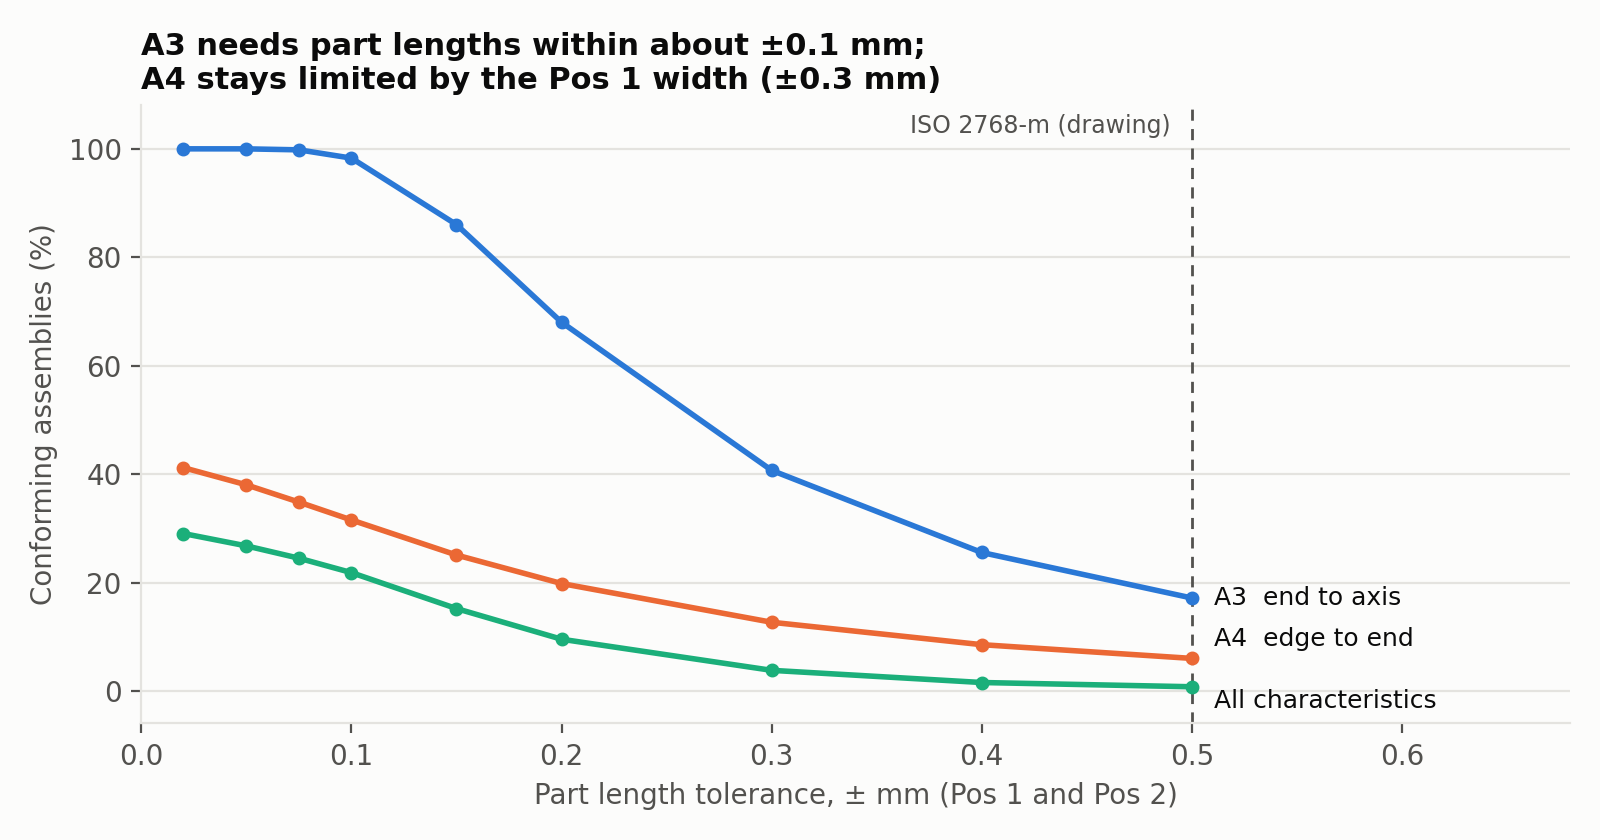
\includegraphics[width=0.85\textwidth]{figures/fig_yield_vs_cut_tolerance.png}
\caption{Conforming assemblies versus the length tolerance of both profiles (self-centring
fixture, Pos~1 paired by height).}
\label{fig:cut}
\end{figure}

\textbf{Recommendation, option 2 with Pos~1 paired by height:}

This gives 100\,\% on A1--A6 and A8. A7 stays at 71\,\%: the remaining height difference between
the paired Pos~1 (0.01\,mm, assumed) and the height variation along each Pos~2 (0.02\,mm, assumed)
already use most of the 0.05\,mm zone. A7 must be checked on real profiles. If the result is
confirmed, the Pos~2 must also be sorted by height, or shims or a machined top face are needed.

%==============================================================================
\section{From simulation to the real cell}
\label{sec:sim2real}

The simulation and the real cell share the cycle logic, not the physics. This section shows how the
code works today (Figure~\ref{fig:arch-sim}), how it would work on the real robots
(Figure~\ref{fig:arch-real}), and what must change.

\subsection{Current architecture: simulation}

Each robot program is a Python generator. At each MuJoCo time step, a scheduler advances both
programs by one step, so the two robots really run in parallel, with exact timing. The programs
compute the inverse kinematics, send the joint and finger targets directly to the simulator and read
back its exact state. For example, when the cycle ``measures'' the part in the gripper
(\code{part\_in\_tcp}), it reads the true position from the simulator; on the real cell, a sensor
is needed. The robots are ideal: a positioning error only exists when it is added on purpose for the
placement study.

The \code{Robot} interface and its MuJoCo backend already exist, but the two-robot cycle does not
use them yet: it talks directly to the simulator to keep exact step-by-step timing. Adapting the
cycle to the interface is the first step towards the real robots.

\begin{figure}[H]
\centering
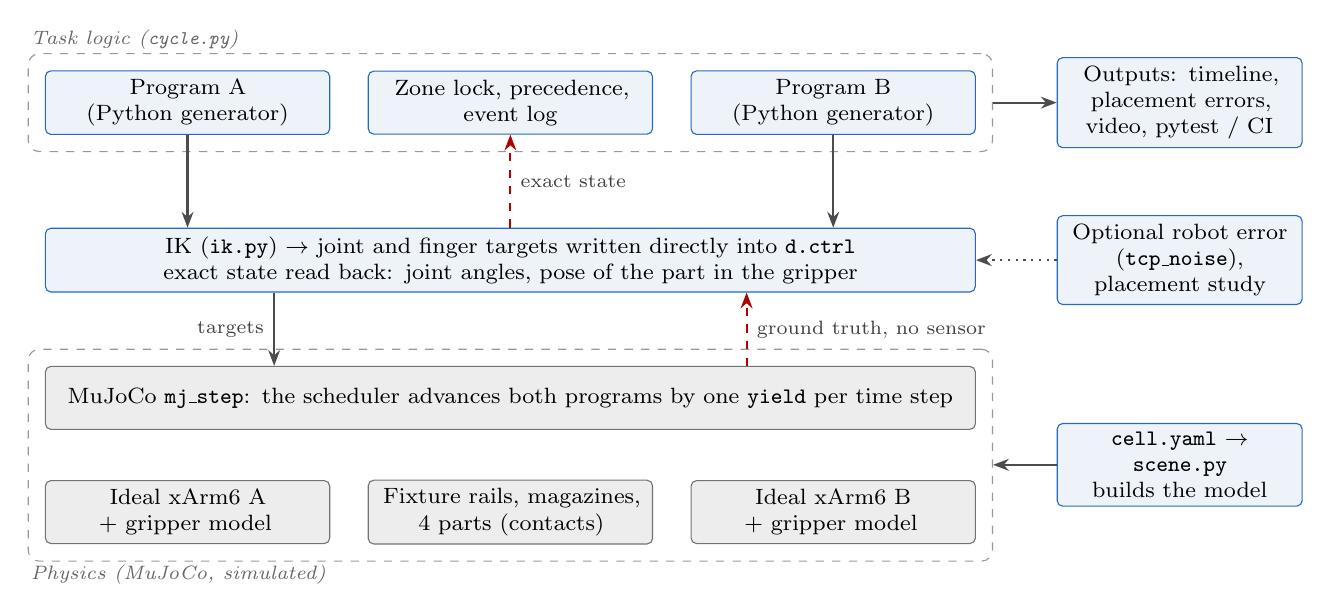
\begin{tikzpicture}
\node[blk,text width=3.4cm] (pA) at (0,0) {Program A\\(Python generator)};
\node[blk,text width=3.4cm] (lk) at (4.1,0) {Zone lock, precedence,\\event log};
\node[blk,text width=3.4cm] (pB) at (8.2,0) {Program B\\(Python generator)};
\node[grp,fit=(pA)(lk)(pB)] (task) {};
\node[grplabel] at (task.north west) {Task logic (\code{cycle.py})};

\node[blk,text width=11.6cm] (acc) at (4.1,-2.0) {IK (\code{ik.py}) $\rightarrow$ joint and finger
targets written directly into \code{d.ctrl}\\exact state read back: joint angles, pose of the part in the gripper};

\node[hw,text width=11.6cm] (stp) at (4.1,-3.75) {MuJoCo \code{mj\_step}: the scheduler advances
both programs by one \code{yield} per time step};
\node[hw,text width=3.4cm] (rA) at (0,-5.2) {Ideal xArm6 A\\+ gripper model};
\node[hw,text width=3.4cm] (fx) at (4.1,-5.2) {Fixture rails, magazines,\\4 parts (contacts)};
\node[hw,text width=3.4cm] (rB) at (8.2,-5.2) {Ideal xArm6 B\\+ gripper model};
\node[grp,fit=(stp)(rA)(fx)(rB)] (sim) {};
\node[grplabel,anchor=north west] at (sim.south west) {Physics (MuJoCo, simulated)};

\node[blk,text width=2.9cm] (out) at (12.6,0) {Outputs: timeline,\\placement errors,\\video, pytest / CI};
\node[blk,text width=2.9cm] (noi) at (12.6,-2.0) {Optional robot error\\(\code{tcp\_noise}),\\placement study};
\node[blk,text width=2.9cm] (cfg) at (12.6,-4.6) {\code{cell.yaml} $\rightarrow$\\\code{scene.py}\\builds the model};

\draw[arr] (pA.south) -- (pA.south |- acc.north);
\draw[arr] (pB.south) -- (pB.south |- acc.north);
\draw[fb] (lk.south |- acc.north) -- node[right,lab]{exact state} (lk.south);
\draw[arr] ([xshift=-3cm]acc.south) -- node[left,lab]{targets} ([xshift=-3cm]stp.north);
\draw[fb] ([xshift=3cm]stp.north) -- node[right,lab]{ground truth, no sensor} ([xshift=3cm]acc.south);
\draw[arr] (task.east) -- (out.west);
\draw[arr,dotted] (noi.west) -- (acc.east);
\draw[arr] (cfg.west) -- (cfg.west -| sim.east);
\end{tikzpicture}
\caption{Current architecture. The task logic is coupled to the simulator: it writes actuator
targets into MuJoCo and reads the exact state back. Blue: code; grey: simulated cell.}
\label{fig:arch-sim}
\end{figure}

\subsection{Target architecture: real cell}

On the real cell, the cycle logic stays the same (programs, zone lock, precedence, event log). Only
what is underneath changes:
\begin{itemize}
  \item \textbf{Robot interface:}\\ each program only uses the \code{Robot} interface, implemented
        by an \code{XArmRobot} backend based on the xArm Python SDK. Each robot has its own thread
        and receives its commands over Ethernet.
  \item \textbf{Controllers:}\\ the xArm controllers are closed: they plan and execute the motion
        and only return joint states and error codes. Their behaviour must therefore be measured,
        not modelled.
  \item \textbf{Calibration:}\\ converts the poses from the cell frame into the frame of each robot.
  \item \textbf{Sensors:}\\ they replace the exact state of the simulation: a camera or laser
        measures the part in the gripper, and digital I/O give the state of the jaws and clamps.
  \item \textbf{Safety and logging:}\\ a safety layer and a data logger complete the cell.
\end{itemize}

\begin{figure}[H]
\centering
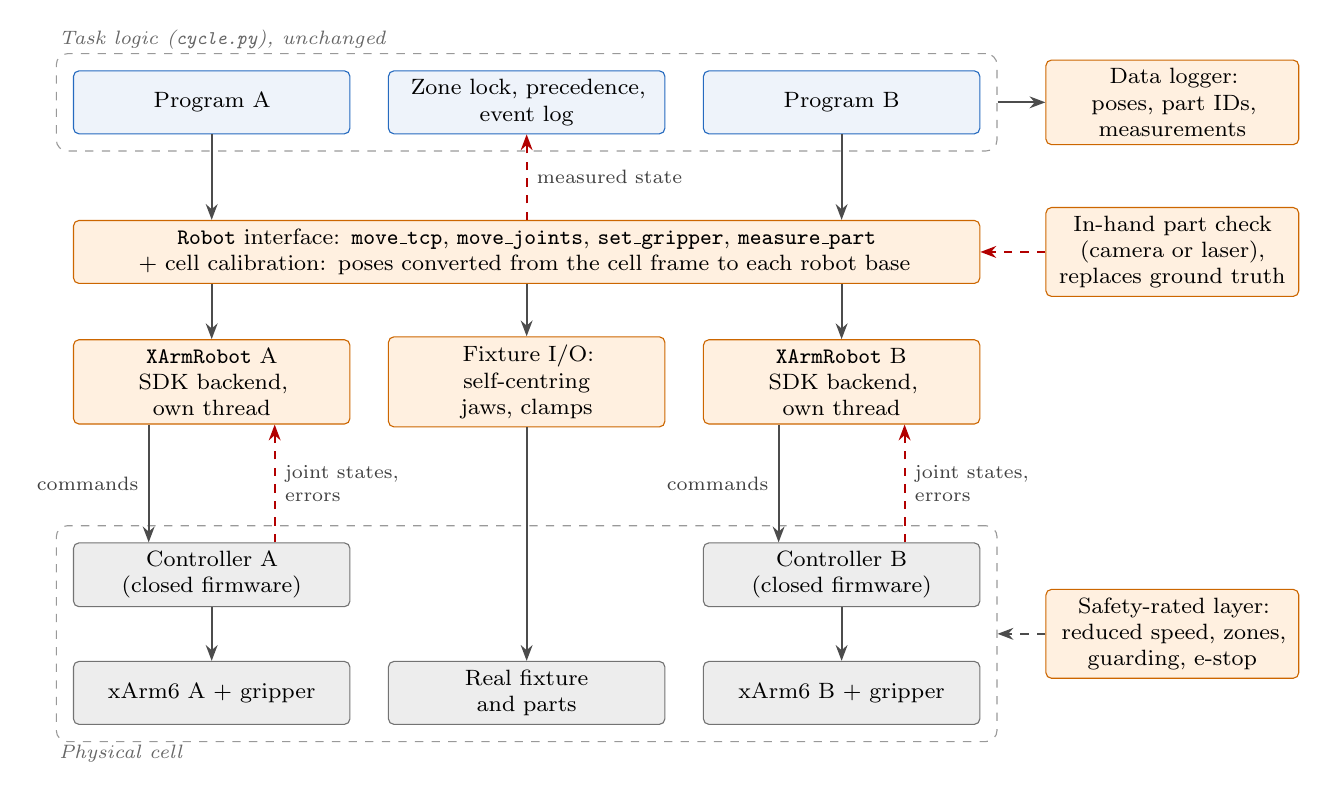
\begin{tikzpicture}
\node[blk,text width=3.3cm] (pA) at (0,0) {Program A};
\node[blk,text width=3.3cm] (lk) at (4.0,0) {Zone lock, precedence,\\event log};
\node[blk,text width=3.3cm] (pB) at (8.0,0) {Program B};
\node[grp,fit=(pA)(lk)(pB)] (task) {};
\node[grplabel] at (task.north west) {Task logic (\code{cycle.py}), unchanged};

\node[new,text width=11.3cm] (rif) at (4.0,-1.9) {\code{Robot} interface: \code{move\_tcp},
\code{move\_joints}, \code{set\_gripper}, \code{measure\_part}\\+ cell calibration: poses converted
from the cell frame to each robot base};

\node[new,text width=3.3cm] (bA) at (0,-3.55) {\code{XArmRobot} A\\SDK backend, own thread};
\node[new,text width=3.3cm] (io) at (4.0,-3.55) {Fixture I/O:\\self-centring jaws, clamps};
\node[new,text width=3.3cm] (bB) at (8.0,-3.55) {\code{XArmRobot} B\\SDK backend, own thread};

\node[hw,text width=3.3cm] (cA) at (0,-6.0) {Controller A\\(closed firmware)};
\node[hw,text width=3.3cm] (cB) at (8.0,-6.0) {Controller B\\(closed firmware)};
\node[hw,text width=3.3cm] (rA) at (0,-7.5) {xArm6 A + gripper};
\node[hw,text width=3.3cm] (fx) at (4.0,-7.5) {Real fixture\\and parts};
\node[hw,text width=3.3cm] (rB) at (8.0,-7.5) {xArm6 B + gripper};
\node[grp,fit=(cA)(cB)(rA)(fx)(rB)] (cell) {};
\node[grplabel,anchor=north west] at (cell.south west) {Physical cell};

\node[new,text width=3.0cm] (log) at (12.2,0) {Data logger:\\poses, part IDs,\\measurements};
\node[new,text width=3.0cm] (sen) at (12.2,-1.9) {In-hand part check\\(camera or laser),\\replaces ground truth};
\node[new,text width=3.0cm] (saf) at (12.2,-6.75) {Safety-rated layer:\\reduced speed, zones,\\guarding, e-stop};

\draw[arr] (pA.south) -- (pA.south |- rif.north);
\draw[arr] (pB.south) -- (pB.south |- rif.north);
\draw[fb] (lk.south |- rif.north) -- node[right,lab]{measured state} (lk.south);
\draw[arr] (bA.north |- rif.south) -- (bA.north);
\draw[arr] (bB.north |- rif.south) -- (bB.north);
\draw[arr] (io.north |- rif.south) -- (io.north);
\draw[arr] ([xshift=-0.8cm]bA.south) -- node[left,lab]{commands} ([xshift=-0.8cm]cA.north);
\draw[fb] ([xshift=0.8cm]cA.north) -- node[right,lab,align=left]{joint states,\\errors} ([xshift=0.8cm]bA.south);
\draw[arr] ([xshift=-0.8cm]bB.south) -- node[left,lab]{commands} ([xshift=-0.8cm]cB.north);
\draw[fb] ([xshift=0.8cm]cB.north) -- node[right,lab,align=left]{joint states,\\errors} ([xshift=0.8cm]bB.south);
\draw[arr] (cA.south) -- (rA.north);
\draw[arr] (cB.south) -- (rB.north);
\draw[arr] (io.south) -- (io.south |- fx.north);
\draw[arr] (task.east) -- (log.west);
\draw[fb] (sen.west) -- (sen.west -| rif.east);
\draw[arr,dashed] (saf.west) -- (saf.west -| cell.east);
\end{tikzpicture}
\caption{Target architecture on the two xArm6. The task logic is the same as in
Figure~\ref{fig:arch-sim}; the simulator is replaced by SDK backends, calibration, sensors and a
safety layer. Blue: existing code; orange: to be implemented; grey: hardware.}
\label{fig:arch-real}
\end{figure}

\subsection{What changes}

\begin{table}[H]
\centering
\caption{Simulation versus real cell.}
\label{tab:sim2real}
\small
\begin{tabularx}{\textwidth}{@{}p{2.7cm} L L@{}}
\toprule
Aspect & Simulation (today) & Real cell\\
\midrule
Motion commands & joint targets written into \code{d.ctrl} at every step & SDK calls; the
controller plans and executes the motion, and its behaviour depends on the control mode\\
Concurrency & one scheduler, one \code{yield} per step & one thread per robot, time-outs, shared
zone lock\\
Frames & robots, fixture and magazines exactly where the model puts them & measured by
calibration; any error propagates to every pose\\
Gripper & modelled fingers, slow force-limited closure & gripper API with its own speed, force
and closing time\\
Part in the gripper & read from the simulator, exact & camera or laser measurement, with its own
uncertainty\\
Fixture & rails with relief pockets & self-centring jaws and clamps driven and read through I/O\\
Robot accuracy & ideal, or error injected on purpose & real accuracy and controller behaviour, to
be measured\\
Errors & an IK failure raises an exception & collisions, lost parts, unreachable poses, controller
faults: detect, stop, recover\\
Safety & not needed & safety-rated functions (reduced speed, zones, guarding, e-stop) designed
from a risk assessment; collision detection as a secondary layer; the zone lock stays task logic\\
\bottomrule
\end{tabularx}
\end{table}

\textbf{Safety:}

The cell is a robot application under ISO~10218-2:2025, which now includes most of the former
ISO/TS~15066 on collaborative applications; the robot itself falls under ISO~10218-1:2025. Using a
``collaborative'' robot does not make the application collaborative: this must be decided by a risk
assessment (ISO~12100) covering the operator who refills the magazines and the zone shared by the
two arms. The zone lock in \code{cycle.py} organises the task; it is not a safety function. On the
real cell, the protection between the robots and of the operator must rely on certified safety
functions designed to ISO~13849-1: reduced speed and safety zones of the controller (after checking
their performance level), plus guarding or a laser scanner on the loading side.

\subsection{Bring-up sequence}

\begin{enumerate}
  \item \textbf{Adapt the cycle to the interface:}\\ rewrite the robot programs to use
        \code{Robot}, and keep running the existing tests in simulation, which remains the
        reference.
  \item \textbf{Write \code{XArmRobot}:}\\ moves, gripper commands, state reading and error
        handling, first tested against a mock of the SDK.
  \item \textbf{Dry run:}\\ run every trajectory without parts and at reduced speed, first in
        visualisation, then on one robot.
  \item \textbf{Calibrate:}\\ measure the position of the two robot bases and of the fixture by
        touching reference points (Section~\ref{sec:valid}, step~2).
  \item \textbf{Characterise the controller:}\\ measure the command latency, the tracking error and
        the repeatability with an external instrument, with and without a part. These values
        replace the datasheet figures in the simulation and in the Monte-Carlo.
  \item \textbf{Increase step by step:}\\ one robot with parts, then both robots with the zone lock,
        and only then higher speeds.
\end{enumerate}

After commissioning, the simulation remains useful: any change to the cycle is first tested in
MuJoCo, then run unchanged on the cell.

%==============================================================================
\section{Validation plan on the real cell}
\label{sec:valid}

Each assumption is replaced by a measurement, starting with those that affect the result the most.
\begin{enumerate}
  \item \textbf{Parts:}\\ measure 20 Pos~1 and 20 Pos~2 (length, width, height at both ends, bow,
        twist) with a calliper and a surface plate, or a CMM. Use these measurements in the
        Monte-Carlo instead of ISO 2768-m and the assumed shape errors. This shows whether precision
        cutting is enough or end machining is needed, and whether A7 can be met.
  \item \textbf{Robot accuracy at the fixture:}\\ for both robots, touch a grid of points on the
        fixture plate with a calibrated probe (or use a laser tracker). This gives the real absolute
        accuracy and the remaining error between the two robot frames, which must stay well within
        the $\pm2$\,mm capture range.
  \item \textbf{Capture:}\\ place each part 50 times with deliberate offsets of up to $\pm2$\,mm and
        $\pm2^\circ$, and measure its final position after the jaws close (dial gauges or laser
        sensors).
  \item \textbf{Assemblies:}\\ build, join and unclamp 30 assemblies, measure A1--A8 on a CMM and
        compute the capability (Cpk) of each characteristic. Compare it with the Monte-Carlo
        prediction.
  \item \textbf{Data:}\\ for each assembly, record the part IDs and dimensions, robot poses, clamp
        states and final measurements, with time stamps, in an open format (CSV or Parquet). This
        allows the model to be updated and drifts to be detected.
\end{enumerate}

%==============================================================================
\section{Assumptions, limitations and next steps}
\label{sec:assump}

The values below are not given by the drawing or a datasheet. They are estimates, grouped in
\code{tolerance/params.py} so that each one can be replaced by a measurement.

\begin{table}[H]
\centering
\caption{Assumed inputs of the simulation and tolerance model.}
\begin{tabularx}{\textwidth}{@{}L l l@{}}
\toprule
Assumption & Value & Used for\\
\midrule
Robot absolute accuracy at the fixture & $\pm1$\,mm ($3\sigma$) per axis, $\pm0.15^\circ$ yaw & S0,
free placement\\
Calibration error between the two robot bases & $\pm0.5$\,mm ($3\sigma$) & S0\\
Part slip in the gripper along its length & $\pm0.5$\,mm ($3\sigma$) & S0\\
Machined fixture features & $\pm0.01$\,mm & S1--S4\\
Self-centring jaw repeatability & 0.003\,mm ($1\sigma$) & S2--S4\\
Lateral bow of a profile, unclamped / clamped & 0.15 / 0.005\,mm ($1\sigma$) & A5, A6\\
Height variation along a Pos~2 & 0.02\,mm ($1\sigma$) & A7\\
Raw contact gap; gap closed by the clamps & 0.10\,mm ($1\sigma$); up to 0.5\,mm & A8\\
Height difference of paired Pos~1 & 0.01\,mm ($1\sigma$) & A7 in S3, S4\\
Precision cutting; end machining & $\pm0.05$\,mm; $\pm0.02$\,mm & S3; S4\\
\bottomrule
\end{tabularx}
\end{table}

\textbf{Limitations:}
\begin{itemize}
  \item The self-centring jaws, the clamps and the joining are not simulated; their effect is only
        estimated with the tolerance model.
  \item The tolerance model treats the parts as perfectly rigid and ignores the bending caused by
        clamping.
  \item The cycle only runs in MuJoCo for now: the interface to send commands to the real xArm6
        (through the UFACTORY Python SDK) is designed but not yet implemented.
  \item Nothing has been tested on the real robots yet.
\end{itemize}

\textbf{Next steps:}
\begin{itemize}
  \item Measure real profiles and use the measured values in the model.
  \item Add the jaws and clamps to the simulation.
  \item Write the code for the real xArm6 and run the cycle on the two robots.
  \item Choose the joining method (tack welding or adhesive) and measure how much it deforms the
        assembly.
  \item An industrial robot is not needed: with this fixture, the xArm6 is accurate enough.
\end{itemize}

\end{document}
